\subsection{Резонансное рождение аксионов в магнитосфере магнитара}
\textcolor{red}{Черновик обзора}
\cite{Weinberg:1975} -- В КХД отсутствие синглетного псевдоголдостановского бозона является хорошо известной проблемой U(1)A. Если бы симметрия U(1)A была спонтанно нарушена, то был бы сгенерирован очень легкий изосинглетный псевдоскалярный голдостановский бозон с массой ? ?3m? согласно киральной теории возмущений

\cite{Dine:1981} -- Простое обобщение модели из~\cite{Quinn:1977}. Аксион всё также легкий и слабо связан с обычной материей. Добавляется одного скалярного поля. Рассмотренный механизм можно реализовать в различных схемах динамического нарушения симметрии.

\cite{Weinberg:1978} и \cite{Wilczek:1978} -- предположили массу аксиона.

\cite{Dine:1983} -- Обсуждаются космологические аспекты очень слабо взаимодействующего аксиона. Упоминается решение проблемы доменных стенок, обсуждаемой Сикиви. Показано, что требование, чтобы аксионы не доминировали над современной плотностью энергии вселенной, дает верхнюю границу константы распада аксиона не более $10^{12}$ ГэВ.

\cite{Preskill:1983} -- Указано новое ограничение на аксион $f_a\gtrsim 10^9$ ГэВ. С учетом того, что плотность энергии аксионного поля не рассеивается быстро, то возникает ограничение $f_a\leqslant10^{12}$ ГэВ. Интерес представляет $f_a\sim 10^{12}$, т. к. такой бездиссипативный, не имеющий давления газ может составлять темную материю.

\cite{Buschmann:2021} -- Показано, что ранее открытый избыток (которого объяснения нет) жесткого рентгеновского излучения $2-8$ кэВ от близлежащих нейтронных звезд может быть объяснено следующим механизмом: Аксионы могут создаваться термически внутри ядра нейтронной звезды, покидать звезду путем их слабого взаимодействия с материей и впоследствии превращаться в рентгеновское излучение в магнитном поле звезды.

\cite{Kim:2010} и \cite{Marsh:2016} -- подробный обзор аксионам.


\textcolor{red}{Конец черновика}

Как было отмечено во Введении к настоящей диссертации, аксион, предложенный Печчеи  и Куинн~\cite{Quinn:1977} для 
решения проблемы сохранения CP инвариантности 
сильных взаимодействий, остается в настоящее время не только самым привлекательным 
решением проблемы CP, но и наиболее вероятным кандидатом на роль холодной темной
материи Вселенной. Поскольку масштаб нарушения симметрии Печчеи-Куинн, $f_a$,
оказывается велик, аксионы очень слабо взаимодействуют с веществом
(константа взаимодействия $f_a^{-1} \lesssim 10^{-8}$\, ГэВ$^{-1}$~\cite{Raffelt:1996}). 
В этой связи возникают определенные трудности
на пути экспериментального обнаружения аксиона.

Как уже неоднократно отмечалось ранее, влияние внешней активной среды на реакции с 
участием элементарных частиц и, в частности,  аксионов,
в зависимости от значений параметров среды (температуры  $T$, 
химического потенциала  $\mu$ или индукции магнитного поля  $B$), может
 как катализировать эти реакции, так и оказывать дополнительное (к $f_a^{-1}$) 
их подавление.  

%
\begin{figure}
\centerline{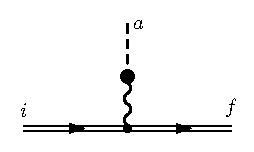
\includegraphics[width=5cm]{fig5_1.eps}}
\caption{Диаграммы Фейнмана для процесса общего вида $i \to 
f+a$. Двойные линии означают, что влияние внешнего поля на начальное и 
конечное состояния учтено точно.}
\label{fig:Diagaxion}
\end{figure}


В таких условиях представляет интерес рассмотреть процесс рождения аксионов   в 
реакции общего вида $i \to f + a$ (диаграмма на рис.~\ref{fig:Diagaxion}), 
где в начальном ($i$) и конечном ($f$) состояниях могут присутствовать 
заряженные компоненты среды. 
На рис.~\ref{fig:Diagaxion} зачерненный
кружок обозначает эффективную вершину $\gamma a$ взаимодействия
(диаграммы на рис.~\ref{fig:vertexaxion}). Нетрудно видеть, что из-за наличия виртуального 
фотона рассматриваемый процесс может иметь резонансный характер. Похожая ситуация
для области, близкой к резонансу, была рассмотрена в работе~\cite{Skobelev:2007} 
на примере
комптоновского рассеяния реликтовых фотонов на электронах и позитронах магнитосферы
магнитара. Однако, как будет показано ниже,  результаты, полученные 
в~\cite{Skobelev:2007}, являются неточными. 

\begin{figure}
\centerline{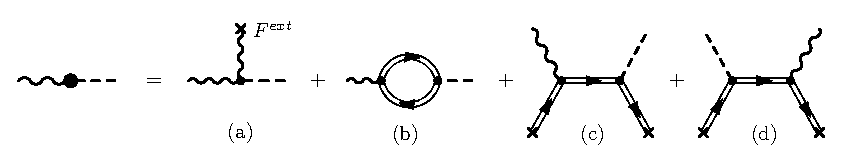
\includegraphics[width=15cm]{fig5_2.eps}}
\caption{ Диаграммы Фейнмана для эффективной вершины $\gamma a$ 
взаимодействия.}
\label{fig:vertexaxion}
\end{figure}



 В существующих аксионных моделях и в присутствии 
внешнего магнитного поля процесс  $i \to f+a$ 
можно описать эффективным лагранжианом вида~\cite{Raffelt:1996} 
(см. также формулы~(\ref{eq:Lel}) и~(\ref{eq:Laxion}) главы~\ref{Sec:1}):
%
\begin{eqnarray}
\label{eq:L1}
&&{\cal L}_{a\gamma}(x) = g_{a\gamma}\tilde F^{\mu \nu} [\partial_{\nu}A_{\mu}(x)] a(x) + 
\\
\nonumber
&& + \frac{g_{af}}{2m_f} 
[\bar \psi_f(x) \gamma^{\mu} \gamma_5 \psi_f(x)] \partial_{\mu} a(x) - 
%\\
%\nonumber
%&+&
 e_f[\bar \psi_f(x) \gamma^{\mu} \psi_f(x)]A_{\mu}(x) \, .
\end{eqnarray}
%
\noindent Напомним, что  $A_{\mu}$ -- четырехмерный потенциал квантованного электромагнитного
поля, $\tilde F^{\mu \nu}$ --  дуальный тензор внешнего поля,  $\psi_f(x)$  и $a(x)$ --  
квантованные фермионное и аксионное поля, 
  $g_{a\gamma} = \alpha \zeta/2\pi f_a$, $\zeta$ --  модельно зависимый 
параметр порядка единицы, 
$g_{af} = C_f m_f/f_a$ -- безразмерная Юкавская константа связи аксионов с 
фермионами с модельно зависимым фактором $C_f$, $e_f$ -- электрический заряд 
фермиона (для электрона $e_f = - e$). 

Исходя из лагранжиана~(\ref{eq:L1}) амплитуда процесса $i \to f + a$ может быть
представлена в следующем виде 
%
\begin{equation}
{\cal M}^a_{i \to f} 
 = - \frac{{\cal M}^{\gamma}_{if} {\cal M}_{\gamma \to a}}
{q'^2 -\varkappa^{(\varepsilon)}(q')}\, , 
\label{eq:M1if}                                                       
\end{equation}
%
\noindent где ${\cal M}^{\gamma}_{if}$ -- амплитуда процесса $i \to f + \gamma$  с 
излучением фотона в конечном состоянии,
%
\begin{equation}
{\cal M}_{\gamma \to a} 
 = i \bar g_{a\gamma} (\varepsilon \tilde F q') 
\label{eq:M2}                                                       
\end{equation}
%
\noindent --  амплитуда перехода фотон $\to$ аксион,  $q'^{\mu} = (\omega',{\bf k}')$ --   
четырехмерный импульс аксиона, $\varkappa^{(\varepsilon)}(q')$ -- собственное значение 
 поляризационного  оператора
фотона, которому соответствует вектор поляризации $\varepsilon_{\alpha}$. Эффективную  
константу аксион-фотонного взаимодействия, $\bar g_{a\gamma}$, можно 
представить в виде трех слагаемых: $\bar g_{a\gamma} = g_{a\gamma} + 
\Delta g^{B}_{a\gamma} + \Delta g^{pl}_{a\gamma}$.    
 Первое слагаемое соответствует взаимодействию 
аксиона с электромагнитным полем, обусловленному аномалией 
Адлера (диаграмма (a) на рис.~\ref{fig:vertexaxion}), второе обусловлено 
взаимодействием аксиона  с фотоном через электронную петлю 
(диаграмма (b) на рис.~\ref{fig:vertexaxion}), а третье --   
рассеянием вперед на электронах и позитронах плазмы (диаграммы (c) и (d) 
на рис.2). Подробный расчет $\Delta g^{B}_{a\gamma}$ и
$\Delta g^{pl}_{a\gamma}$ был сделан ранее в работах~\cite{Mikheev:1999} 
и~\cite{Mikheev:2006} соответственно. 
 Здесь мы отметим только, что для корректного вычисления величины $\Delta g^{B}_{a\gamma}$  
в ней необходимо 
 произвести вычитание, соответствующее аномалии Адлера~\cite{Mikheev:1999}. 
Этот факт, в 
частности, не был учтен в работе~\cite{Skobelev:2007}, что является одной из причин  
ошибочности полученных там результатов.

Далее представим $\varkappa^{(\varepsilon)}(q')$ в виде    
$\varkappa^{(\varepsilon)} = \Re - i\Im$, 
где $\Re = Re (\varkappa)$  реальная, а $\Im =  Im (\varkappa)$  мнимая части 
поляризационного оператора. Последняя обусловлена процессами поглощения и 
излучения фотонов в плазме и,
согласно~\cite{Weldon:1983}, следующим образом выражается через полную 
ширину рождения фотона, $\Gamma_{cr}$: 
%
\begin{eqnarray}
\label{eq:I1}                                                       
\Im = \omega' \left (e^{\omega'/T} - 1 \right ) \Gamma_{cr} ,  \quad 
%\\
%\nonumber 
\Gamma_{cr} = \sum_{i,f} \int  |{\cal M}^{\gamma}_{if}|^2 d\Phi_{if} ,
\end{eqnarray}
%
\noindent где $d\Phi_{if}$ --  элемент фазового объема состояний $i$ и $f$ для процесса 
$i \to f + \gamma$ с учетом соответствующих функций распределения,  
и сумма берется по всем возможным начальным и конечным состояниям. 

С учетом вышесказанного, аксионная светимость за счет всевозможных реакций с участием 
частиц плазмы может быть представлена  в виде 
%
\begin{equation}
Q = \sum_{i,f} \int d\Phi_{if} \, d\Phi' \, \omega' 
|{\cal M}^{\gamma}_{if}|^2 \, ,
\label{eq:Qa0}                                                       
\end{equation}
%
\noindent где $d\Phi' = \frac{d^3 k'}{(2\pi)^3 2 \omega'}$  фазовый объем аксиона. 

С учетом~(\ref{eq:M1if}) и~(\ref{eq:I1}) $Q$ примет вид
%
\begin{equation}
Q = \int  \frac{d\Phi' \, |{\cal M}_{\gamma \to a}|^2}{e^{\omega'/T} - 1} \, 
\frac{\Im
} 
{(q'^2 -\Re)^2 + \Im^2} \, .
\label{eq:Qa1}                                                       
\end{equation}
%

Как видно из~(\ref{eq:Qa1}), наиболее существенный вклад в аксионную светимость будет
давать область резонанса, т.е. окрестность точки пересечения дисперсионных кривых
аксиона $q'^2 = m_a^2$ и фотона, $q'^2 = \Re$, так 
что фотон становится реальным. В окрестности резонанса часть подынтегрального выражения
в~(\ref{eq:Qa1}) можно интерполировать $\delta$-функцией:  
%
\begin{equation}
 \frac{\Im}
{(q'^2 -\Re)^2 + \Im^2} \simeq \pi \, \delta(q'^2 -\Re) \, .
\label{eq:Del1}
\end{equation}
%
\noindent Воспользовавшись свойствами $\delta$-функции, перепишем~(\ref{eq:Del1})
 в виде  
%
\begin{equation}
 \frac{\Im}
{(q'^2 -\Re)^2 + \Im^2} \simeq \pi \, 
\int \frac{d^3 k}{2 \omega} Z_{\varepsilon} \delta^4 (q-q') \, ,
\label{eq:Del2}
\end{equation}
%
\noindent где  $Z_{\varepsilon}^{-1} = 1-\frac{\partial \Re}{\partial \omega^2}$ 
соответствует перенормировке волновой функции фотона.


 С учетом~(\ref{eq:Del2}) cветимость~(\ref{eq:Qa1}) примет вид 
%
\begin{eqnarray}
\label{eq:Qa2}
Q &\simeq&  (2\pi)^4 \, 
\int \frac{d^3 k}{2 \omega (2\pi)^3} \,\frac{\omega}{e^{\omega/T} - 1} \times
\\
\nonumber 
&\times& \int \frac{d^3 k'}{2 \omega' (2\pi)^3}\, Z_{\varepsilon} 
|{\cal M}_{\gamma \to a}|^2 \delta^4 (q-q') \, .
\end{eqnarray}
%
\noindent Полученное выражение в точности соответствует формуле для аксионной светимости  
в процессе $\gamma \to a$. Таким образом, аксионная светимость в 
области резонанса за счет всевозможных  
реакций с участием частиц среды 
  однозначно выражается через светимость перехода фотон $\to$ 
аксион.


После интегрирования с $\delta$-функциями светимость приводится к виду
%
\begin{eqnarray}
Q =  \frac{\bar g_{a\gamma}^2 (\beta)^2}{32 \pi^2 \alpha} \, 
\int_{-1}^1 \frac{dx}{e^{\omega/T}-1} \, 
\frac{Z_{\varepsilon} k 
(\varepsilon \tilde \varphi q)^2}{\left |1-\frac{d\omega^2}{dk^2}\right |}\bigg |_{k=k^*}\, .
\label{eq:Qa3}
\end{eqnarray}
%

\noindent Здесь $x = \cos{\theta}$, $\theta$ --  угол 
между направлением импульса фотона и магнитным полем, $k^* = k^*(\theta)$ --  
 корень уравнения $\omega^2 (\vec k) = m_a^2+k^2$. 
% $\tilde \varphi_{\alpha \beta} = \tilde F_{\alpha \beta}/B$.


Дальнейшее вычисление светимости будет существенно зависеть от характеристик плазмы, 
определяющих, в конечном итоге, дисперсионные свойства фотонов. Здесь мы остановимся 
на двух частных случаях.

i) Слабо замагниченная плотная плазма,  $m_a^2 \ll \beta \ll T^2 , \mu^2$. В этом 
случае в качестве $\varepsilon_\alpha$ будет выступать вектор поляризации продольного 
плазмона
%
\begin{eqnarray}
\varepsilon_\alpha = \sqrt{\frac{q^2}{(uq)^2-q^2}}\, 
\left (u_\alpha - \frac{(uq)}{q^2}\, q_\alpha \right ) , 
\end{eqnarray}
%
где $u_\alpha$ -- 4-скорость плазмы. Светимость~(\ref{eq:Qa3}) примет простой вид
%
\begin{eqnarray}
Q =  \frac{\bar g_{a\gamma}^2 (\beta)^2}{48 \pi^2 \alpha} \, 
 \frac{(k^*)^3}{e^{k^*/T}-1} \, 
\label{eq:Qa4}
\end{eqnarray}
%

\noindent 
в полном согласии с результатом работы~\cite{MRV:1998}. Отметим, что в данном пределе 
 величина $k^*$ не зависит от $\theta$, а определяется только параметрами плазмы.


ii) Сильно замагниченная нерелятивистская холодная плазма  $\beta \gg m^2$, $\mu^2 \gg T^2$. Здесь %\newline   
$\varepsilon_\alpha = 
(q \tilde \varphi)_\alpha/\sqrt{q^2_{\mprl}}$, 
$\Re \simeq (q \tilde \varphi \tilde \varphi q) \left (\frac{\omega_p^2(1+\xi)}{\omega^2} -
\xi \right )$, и плазменная частота $\omega_p$   
следующим образом связана с концентрацией электронов:  $\omega^2_p = 4\pi \alpha n/m$; $\xi = (\alpha/3\pi)(B/B_e)$. 
Кроме того, в рассматриваемом пределе 
$\bar g_{a\gamma} \simeq g_{a\gamma}$. Однако,  
в отличие от случая слабо замагниченной плазмы, светимость до конца интегрируется
лишь в некоторых частных случаях:

\begin{itemize} 

\item масса аксиона --  наименьший параметр задачи, т.е. 
$\omega_p, \,T \gg m_a$ (например, рождение легких, с массой меньшей, чем 
$10^{-5}$\,эВ, аксионов в магнитосфере
магнитара).  % (см. формулу~(\ref{eq:n1}))). 
В этом случае 
$k^* \simeq \omega_p \sqrt{1+1/\xi}$ и светимость~(\ref{eq:Qa3}) примет вид
%
\begin{eqnarray}
\label{eq:Qa5a}
Q &\simeq&  \frac{g_{a\gamma}^2 (\beta)^2}{16 \pi^2 \alpha} \,
\omega_p^3 \frac{(1+\xi)^{3/2}}{\xi^{5/2}}\times
\\
\nonumber 
&\times& \left (\exp{\left [\frac{\omega_p}{T} 
\sqrt{1+\frac{1}{\xi}}\, \right ]}-1 \right )^{-1} \, .
\end{eqnarray}
%


\item $\omega_p \gg T \sim m_a$. Анализ показывает, что в этом 
случае интеграл в~(\ref{eq:Qa3}) набирает
свою величину в области $x\simeq 1$, и, следовательно, $k^* \simeq \omega_p $.
  Тогда светимость примет вид
%
\begin{eqnarray}
\label{eq:Qa5b}
Q &\simeq&  \frac{g_{a\gamma}^2 (\beta)^2}{16 \pi^2 \alpha} \, T m_a^2  \, 
e^{-\omega_p/T} \, .
\end{eqnarray}
%

\end{itemize}

Кроме светимости представляет самостоятельный интерес оценка количества аксионов,
рождаемых в магнитосфере магнитара в единице объема за единицу времени с 
помощью рассмотренного выше резонансного
механизма, поскольку аксион является одним из основных кандидатов в составляющие
холодной темной материи. Аналогично~(\ref{eq:Qa3}), (\ref{eq:Qa5a}) 
и~(\ref{eq:Qa5b}) получаем: 
%
\begin{eqnarray}
\frac{dN}{dt dV} =  \frac{g_{a\gamma}^2 (\beta)^2}{32 \pi^2 \alpha} \, 
\int_{-1}^1 \frac{dx}{e^{\omega/T}-1} \, 
%\frac{k}{\omega} \, 
\frac{k Z_{\varepsilon} 
(\varepsilon \tilde \varphi q)^2}{\omega 
\left |1-\frac{d\omega^2}{dk^2}\right |}\bigg |_{k=k^*}\, ,
\label{eq:Na0}
\end{eqnarray}
%

%
\begin{eqnarray}
\label{eq:Na1}
\frac{dN}{dt dV} &\simeq&  \frac{g_{a\gamma}^2 (\beta)^2}{16 \pi^2 \alpha} \,
\omega_p^2 \frac{1+\xi}{\xi^{2}}\times
\\
\nonumber 
&\times& \left (\exp{\left [\frac{\omega_p}{T} 
\sqrt{1+\frac{1}{\xi}}\, \right ]}-1 \right )^{-1} \, , \quad \omega_p,\, T \gg m_a,
\end{eqnarray}
%

%
\begin{eqnarray}
\label{eq:Na2}
\frac{dN}{dt dV} &\simeq&  \frac{g_{a\gamma}^2 (\beta)^2}{16 \pi^2 \alpha} \,
\frac{T m_a^2}{\omega_p}  \, e^{-\omega_p/T} \, , \quad \omega_p \gg T \sim m_a.
\end{eqnarray}
%



В частности, для числа аксионов, рождаемых реликтовым излучением 
($T \sim m_a \sim 10^{-3}$\,эВ), при  
 минимальной  концентрации плазмы ($\sim 10^{15}$\,см$^{-3}$), при которой все еще 
 реализуется  резонансный механизм $(\omega_p \gtrsim  m_a)$ и величине магнитного поля 
 $B=100B_e$, получаем из~(\ref{eq:Na0})  
следующую максимальную оценку $dN/(dV dt)\sim 10^{10}$ штук в см$^{-3}$ за секунду. 
 Таким образом, в объеме магнитосферы магнитара 
 ($\sim 10^{19}$\,см$^3$), заполненной сильным магнитным полем,  рождается за секунду 
 $10^{29}$ аксионов. Оценивая в самом оптимистичном варианте 
 число магнитаров в Галактике $\sim 10^6$, получаем, 
 что за $\sim 10^9$ лет они произведут $\sim 10^{51}$ аксионов, и, следовательно, 
 концентрация  аксионов в Галактике должна быть  $n_a \sim 10^{-21}$\,см$^{-3}$. Это число
 можно сравнить, например, с концентрацией барионов $n_b \sim 10^{-7}$\,см$^{-3}$ $\gg n_a$.  
 Следовательно, утверждение автора~\cite{Skobelev:2007} о том, что <<окрестности 
 магнитных нейтронных 
 звезд с полями $B \gg B_e$ могут являться мощными генераторами по преобразованию 
 реликтового излучения в аксионную составляющую холодной скрытой массы>> не является 
 верным.
 
 %%%%%%%%%%%%%%%%%%%
 %                                                   %
 %                                                   %
 %%%%%%%%%%%%%%%%%%%
 
 
 \subsection{Резонансный механизм рождения $e^+e^-$ пар  в полярной шапке магнитара}
Наконец, рассмотрим   реакцию $\gamma e \to e e^+e^-$, в которой могут иметь место одновременно два резонанса: 
на виртуальном фотоне и на виртуальном электроне, что особенно важно для актуальной в настоящее время  
проблемы  описания особенностей 
радиоизлучения некоторых магнитаров~\cite{Malofeev:2005r, Malofeev:2005,
Duncan:1995,Thompson:1996,Thompson:2002}.  

Согласно общепринятой модели, для 
формирования радиоизлучения  в радиопульсаре необходима эффективная генерация 
электрон-позитронной плазмы в его магнитосфере~\cite{Ruderman:1975}, 
причем механизмы рождения $e^+e^-$-пар 
в радиопульсарах хорошо известны (см., например,~\cite{Klepikov:1954,Erber:1966}).  

%
\begin{figure}
\centerline{
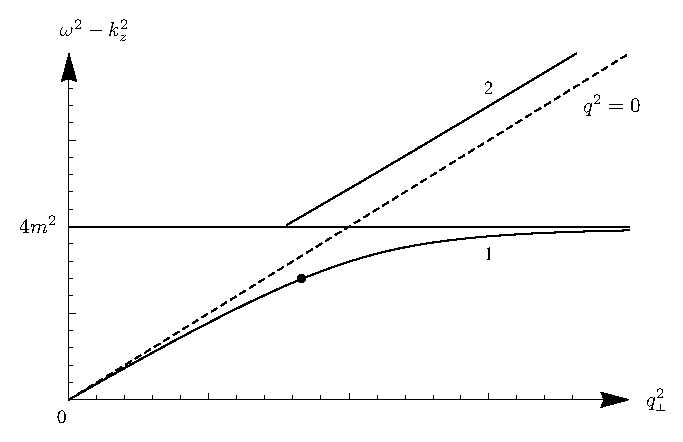
\includegraphics[width=12cm]{fig5_3.eps}}
\caption{ Закон дисперсии фотона в сильном магнитном поле. 
Точкой на дисперсионной кривой 
показано положение фотона, рождающегося в реакции  $e \gamma \to e \gamma$.
 Цифры 1 и 2 обозначают дисперсионные кривые в областях ниже и выше 
порога рождения $e^+e^-$-пар.}
\label{fig:dispersion}
\end{figure}

В модели магнитосферы магнитара рождение $e^+e^-$-пар происходит в два 
этапа~\cite{Beloborodov:2007}. Ускоренная вдоль магнитного поля 
заряженная частица (электрон или позитрон)  
резонансно конвертирует мягкий рентгеновский 
фотон в жесткий, который впоследствии, как предполагается, 
после набора угла между импульсом фотона и направлением 
магнитного поля (так называемый питч-угол), 
должен распадаться на электрон-позитронную пару.  Однако в действительности этого не происходит, так как 
в сильном магнитном поле существенными становятся 
дисперсионные свойства фотона (см. раздел~\ref{Sec:2.2}  и рис.~\ref{fig:dispersion}). Такой фотон, рожденный 
в реакции $e\gamma \to e \gamma$ с энергией и импульсом, удовлетворяющими соотношению 
$\omega^2-k_z^2 < 4m^2$ (магнитное поле направлено по оси $z$), в процессе распространения 
в магнитном поле будет все время оставаться на дисперсионной ветви 1 и не сможет преодолеть 
зазор между ветвями 1 и 2 с рождением $e^+e^-$-пары, если 
величина магнитного поля $B \gtrsim 0.1 B_e$~\cite{Shabad:1975,ShabUsov:1982,ShabUsov:1985}, 
что заведомо выполняется в магнитарах. 
При достаточно больших $q^2_{\mprp}$ 
такой фотон может лишь перейти на асимптотически больших расстояниях 
в позитроний -- связанное состояние $e^+e^-$-пары. 



В связи с этим представляет интерес рассмотреть альтернативный механизм  рождения 
$e^+e^-$-пар в магнитосфере магнитара. В качестве такого механизма может выступать 
комптоноподобный процесс $\gamma e \to e e^+e^-$, где 
под $e$ в дальнейшем понимается электрон или позитрон. 
Основное преимущество такой реакции по сравнению с принятой 
моделью состоит в том, что рождение пары происходит практически мгновенно в точке взаимодействия 
начальных фотона и электрона 
(в действительности этот масштаб имеет порядок комптоновской длины волны электрона). При таком 
подходе эффект захвата фотона полем становится несущественным. 
Вместе с тем, с помощью 
реакции $\gamma e \to e e^+e^-$ возможно за короткие времена заполнить ограниченную область 
 достаточно плотной 
$e^+e^-$-плазмой, как, например, 
в процессе гигантской вспышки источника мягких повторяющихся 
гамма всплесков (SGR).

%
\begin{figure}
\centerline{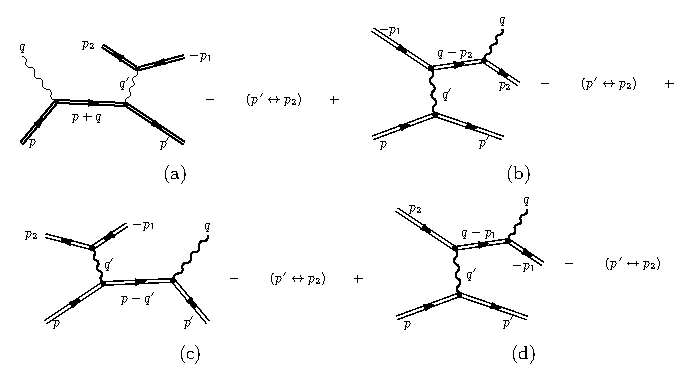
\includegraphics[width=17cm]{fig5_4.eps}}
\caption{Диаграммы Фейнмана для процесса $\gamma + e^{-} \to e^{-} + e^{+}e^{-}$. 
Двойные линии означают, что влияние внешнего поля на начальное и 
конечное состояния учтено точно.}
\label{fig:Diag}
\end{figure}

%\section{Амплитуда перехода $\gamma e \to e e^+ e^-$}



Процесс рождения электрон-позитронных пар в реакции $\gamma e \to e e^+ e^-$  
описывается восемью диаграммами Фейнмана (см. рис.~\ref{fig:Diag}). Нетрудно 
видеть, что резонанс на виртуальном электроне имеет место только в $s$-канальных 
диаграммах  (рис.~\ref{fig:Diag} $a$ 
и соответствующая диаграмма с перестановкой 
$p^{\, \prime} \leftrightarrow p_2$). Тем  не менее, даже с учетом резонанса 
поставленная 
задача будет иметь достаточно громоздкий вид, поскольку заряженные фермионы могут занимать 
произвольные уровни Ландау. Однако в приложении к магнитарам данную проблему можно 
значительно упростить. Действительно, рассмотрим ситуацию, когда  
электрон, ускоренный в электрическом зазоре полярной шапки 
магнитара, сталкивается с гамма-квантом из равновесной термальной бани, образованной излучением 
рентгеновских фотонов с поверхности нейтронной 
звезды. В такой постановке задачи мы будем иметь следующую иерархию параметров:   
$T^2 \ll m^2 \ll \beta \ll E^2$. Кроме того, электрон, до ускорения находившийся на основном 
уровне Ландау $(\ell = 0)$, двигаясь вдоль силовой линии 
магнитного поля, остается все время на основном уровне. 
(Мы рассматриваем небольшую окрестность полярной шапки, где электрическое, 
$\vec {\cal E}$, и магнитное $\vec B$ поля 
коллинеарны и при этом $|\vec {\cal E}| \ll |\vec B|$~\cite{Beloborodov:2007}.) 
 Не нарушая общности будем считать, что  рассеянный
электрон и электрон и позитрон пары также будут находиться на основном уровне Ландау 
 с $\ell^{\, \prime} = n_1 = n_2 = 0$.  Действительно,  как было показано в разделе~\ref{Sec:5.3.1},  
полученный результат для коэффициента поглощения электрона не будет зависеть от состояния конечных частиц, 
а будет определяться только начальными состояниями электрона и фотона.

С учетом этого замечания  
$S$ -- матричный элемент  процесса $\gamma e \to e e^+ e^-$  может быть записан 
в виде:   
%
\beq
\label{eq:S1}
&&{\cal S}_{\gamma e \to e e^+ e^-} = 
(\ii e)^3 \int d^4 X d^4 Y d^4 Z 
\times 
\\[3mm]
\nonumber
&&\times
\big \{ \bar \Psi^{-}_{p',0}(Y) \gamma_{\beta} 
\hat S(X,Y) \hat A(X) \Psi^{-}_{p,0}(X) \bar \Psi^{-}_{p_2,0}(Z) \gamma_{\mu} \Psi^{+}_{p_1,0}(Z) -  
\\[3mm]
\nonumber
&&-\bar \Psi^{-}_{p_2,0}(Y) \gamma_{\beta} 
\hat S(X,Y) \hat A(X) \Psi^{-}_{p,0}(X)  
\bar \Psi^{-}_{p',0}(Z) \gamma_{\mu} \Psi^{+}_{p_1,0}(Z) \big \}
G_{\beta \mu} (Z-Y) \, ,
\eeq

\noindent где  $p^{\mu} = (E,{\bf p})$ -- 4-импульс начального электрона, 
$p'^{\mu} =(E^{\, \prime}, {\bf p}^{\, \prime})$ -- 4-импульс конечного электрона,  
$p_2^{\mu} =(E_2, {\bf p}_2)$  и  $p_1^{\mu} =(E_1, {\bf p}_1)$ -- 4-импульсы 
электрона и позитрона пары соответственно, 
$X^{\mu} = (X_0, X_1, X_2, X_3)$, $Y^{\mu} = (Y_0, Y_1, Y_2, Y_3)$, $Z^{\mu} = (Z_0, Z_1, Z_2, Z_3)$,
%
\beq
A_\mu (X) = \frac{\varepsilon_\mu (q) e^{-\ii(qX)}}{\sqrt{2\omega V}} \, ,  
\eeq
%
\noindent -- квантованное поле начального фотона, 
несущего 4-импульс $q^{\mu} =(\omega, {\bf k})$.   
%
\beq
\label{eq:phot_prop}
&&G_{\beta \mu} (Z) = \int \frac{\dd^4 q^{\, \prime}}{(2 \pi)^4} \eee^{-\ii(q^{\, \prime}Z)} 
{\cal G}_{\beta \mu} (q^{\, \prime})\, , %\quad   
\\
\nonumber
&&{\cal G}_{\beta \mu} (q^{\, \prime}) = 
\sum_{\lambda = 1}^3 \,
\frac{b_{\beta}^{(\lambda)} b_{\mu}^{(\lambda)}}{(b^{(\lambda)})^2} 
\,\frac{ - i}
{q^{\, \prime 2} - \varkappa^{(\lambda)}(q^{\, \prime})},
\eeq
% 
\noindent -- фурье-образ пропагатора виртуального фотона в базисе из 4-векторов $b_{\alpha}^{(\lambda)}$, 
определяемых согласно~(\ref{eq:basis}),  
%$b_{\alpha}^{(\lambda)}$: $b_\alpha^{(1)} = (q^{\, \prime} \varphi)_\alpha$, 
% $b_\alpha^{(2)} = (q^{\, \prime} \tilde \varphi)_\alpha$,  
% $b_\alpha^{(3)} = q^{\, \prime 2}(q^{\, \prime} \varphi \varphi)_\alpha - 
%(q^{\, \prime}\varphi \varphi q^{\, \prime}) q^{\, \prime}_\alpha$, 
 $\varkappa^{(\lambda)}(q^{\, \prime})$ -- собственные значения поляризационного оператора 
фотона, соответствующие векторам  $b_{\alpha}^{(\lambda)}$ (см., 
например,~\cite{Shabad:1975} и раздел~\ref{Sec:2.2}), 
$\Psi^{\mp}_{p,0}(X)$ 
-- волновые функции электрона (позитрона) во внешнем магнитном поле,  находящихся на основном уровне Ландау 
и определяемые формулами~(\ref{eq:psip1}) и~(\ref{eq:psim1})  приложения~\ref{Sec:app_d}, $\hat S(X,Y)$ -- 
пропагатор электрона, определяемый формулами~(\ref{eq:propagator_sum_n}) -- (\ref{eq:propagator_ns}). 
%Поле позитронов описывается с помощью  отрицательно частотного решения, волновая функция которого получается 
%сменой знака у величин $E, p_y, p_z$. 
 
%Используя  пропагатор электрона в 
%следующей форме~\cite{KuznOkrug:2011} (см. приложение):  
%

                                                      
После интегрирования~(\ref{eq:S1}) по $d^4X$, $d^4Y$ и $d^4Z$ мы получим 
%
\beq
\label{eq:SV2}                                  
{\cal S}_{\gamma e \to e e^+ e^-} =   
\frac{\ii (2\pi)^3 \delta^3 (\ldots) {\cal M}_{\gamma e \to e e^+ e^-}}
{\sqrt{2\omega V 2 E L_y L_z 2 E^{\, \prime} L_y L_z 2 E_1 L_y L_z 2 E_2 L_y L_z}}\, 
 \, , 
\eeq
\noindent где    $\delta^3 (\ldots) \equiv \delta (P_0 - E^{\, \prime}-E_1-E_2) 
\delta (P_y - p^{\, \prime}_y - p_{1y}-p_{2y}) 
\delta (P_z - p^{\, \prime}_z -p_{1z}-p_{2z})$, $P_\alpha \equiv (p+q)_\alpha , 
\,\, \alpha =0,2,3$.
%


Амплитуда процесса $\gamma e\to e e^+e^-$, 
таким образом, может быть представлена в виде
%
\beq
\nonumber
&&{\cal M}_{\gamma e\to e e^+e^-} \simeq - \ii \frac{2 \sqrt{2}e^3 m^2}{\pi}  
\sum \limits_{n=0}^{\infty}
\; \int \limits^{\infty}_{-\infty} 
\frac{d q^{\, \prime}_x}{q^{\, \prime 2} - \varkappa^{(2)}(q^{\, \prime})} \; 
\exp \left [-\frac{\ii (q \varphi q^{\, \prime})}{2e B} \right ] \times
\\[3mm]
\label{eq:M11}
&&\times
\exp \left [-\frac{\ii(q_x-q^{\, \prime}_x) (p_y+p^{\, \prime}_y)}{2e B} \right ] 
\exp \left [\frac{\ii q^{\, \prime}_x(p_{1y}-p_{2y})}{2e B} \right ] \times 
\\[3mm]
\nonumber
&&\times 
\exp \left [- \frac{2q^{\, \prime 2}_{\mprp}+
q^2_{\mprp}}{4\beta} \right] \; \frac{1}{n!} \left (\frac{(q\Lambda q^{\, \prime})-\ii 
(q\varphi q^{\, \prime})}
{2\beta} \right )^n  
 \times 
\\[3mm]
\nonumber
&&\times \frac{(pq^{\, \prime})_{\mprl} [(pq)_{\mprl} + (p^{\, \prime}q)_{\mprl}]}
{\left (P^2_{\mprl} - m^2 - 2e Bn + \ii P_0 \Gamma_n \right ) 
\sqrt{q^2_{\mprl}q^{\, \prime 2}_{\mprl} 
[(pp^{\, \prime})_{\mprl} + m^2]}}_{\bigg |\substack{
q^{\, \prime \alpha}_{\mprl} = p^{\alpha}_{1 \mprl} + p^{\alpha}_{2 \mprl}\\ 
 q^{\, \prime}_y = p_{1y}+p_{2y}}} -   
\\[3mm]
\nonumber
&&-(p^{\, \prime} \leftrightarrow p_2)\, .
\eeq

Здесь необходимо сделать следующее замечание. Мнимая часть пропагатора электрона, связанная с 
полной шириной поглощения электрона соотношением~(\ref{eq:I_Sigma}), вообще говоря,  зависит 
от поляризационного состояния электрона,  
и только в пределе сильного поля, $B \gg B_e$, эта зависимость становится несущественной, что 
позволяет провести суммирование по поляризациям электрона и представить амплитуду в виде~(\ref{eq:M11}).


Для корректного описания рассматриваемого процесса вблизи резонанса необходимо также  
учесть полную ширину процесса поглощения электрона, $\Gamma_{n}$, основной вклад в которую  
будет давать переход $e_n \to \gamma + e_{n'}$. Исходя из результатов 
работ~\cite{Latal:1986,Kuznetsov:2003}, величина $P_0\Gamma_{n}$ в пределе сильного поля и ультрарелятивистских 
электронов может быть представлена в следующем виде:
%
\beq
\label{eq:width}
&&P_0 \Gamma_n \simeq \alpha \beta \sum^{n-1}_{n'=0} 
\int \limits^{(\sqrt{n}-\sqrt{n'})^2}_0 
\frac{d x}{\sqrt{(n+n'-x)^2 - 4 n n'}}\, \times
\\
\nonumber 
&&\times \{(n+n'-x)[{\cal I}^2_{n, n'-1} (x) +
{\cal I}^2_{n-1, n'} (x)] -
4 \sqrt{n n'} {\cal I}_{n, n'} (x){\cal I}_{n-1, n'-1} (x) \}\, . 
\eeq


Определяя стандартным путем коэффициент поглощения электрона в 
равновесном фотонном газе, имеющем температуру $T$, получим
%
\beq
\label{eq:w1}
W = \int \frac{\delta^3 (\ldots) |{\cal M}|^2}
{2^5 (2 \pi)^6 \omega E E^{\, \prime} E_{1} E_{2}}\, 
\frac{d^3q}{e^{\omega/T}-1} 
d p^{\, \prime}_y d p^{\, \prime}_z d p_{1y} d p_{1z} d p_{2y} d p_{2z}\, . 
\eeq

Как уже отмечалось, основной вклад в амплитуду будут давать области резонанса, так что 
мы можем заменить часть подынтегрального выражения в~(\ref{eq:w1}) 
$\delta$-функцией
%
\beq
\label{eq:delta1}
\frac{1}{(P^2_{\mprl} - m^2 - 2e Bn)^2 + P_0^2 \Gamma_n^2} \simeq 
\frac{\pi}{P_0 \Gamma_n}
\delta (P^2_{\mprl} - m^2 - 2e Bn) \, .
\eeq


Вводя новые переменные $y = q^{\, \prime 2}_{\mprp}/{\beta}$ и $z = q^{\, \prime}_z/E$, получим 
в нашем приближении  
$q^{\, \prime 2}_{\mprl} \simeq 2 \beta z$, $(q-q^{\, \prime})^2_{\mprl} \simeq - m^2 z^2/(1-z)$. 
Кроме того, лидирующий вклад от уровней Ландау виртуального электрона будет определяться только уровнем с 
$n=1$, вклады высших уровней оказываются подавлены температурой.  В этом случае ширина 
поглощения электрона принимает особенно 
простой вид: $P_0\Gamma_1 \simeq \alpha \beta (1-e^{-1})$.
После интегрирования с $\delta$-функциями  выражения~(\ref{eq:w1}), с учетом вышесказанного, 
получим
%
\beq
\label{eq:W18}
W &\simeq& \frac{\alpha^2 T}{2 \pi (1-e^{-1})}\, \left (\frac{m}{E} \right )^2 
\ln{\left (1- e^{-\frac{\beta}{2ET}} \right )^{-1}} 
\int \limits_{2B_e/B}^{1} d z
\times
\\
[3mm] \nonumber
&\times&\int \limits_{0}^{\infty} 
\frac{d y y e^{-y} }{z^2(2z-y)^2 + 4 \alpha^2 (B_e/B)^2 e^{-y}}\, .
\eeq


Нетрудно видеть, что и здесь часть подынтегрального выражения можно приближенно заменить  
$\delta$-функцией: 
%
\beq
\label{eq:photres}
\frac{1}{z^2(2z-y)^2 + 4 \alpha^2 (B_e/B)^2 e^{-y}} 
\simeq \frac{\pi e^{y/2}}{2\alpha} \, 
\frac{B}{B_e}\, \delta(2z^2-yz) \, , 
\eeq

\noindent т.е. в процессе $e \gamma \to e e^+e^-$ в пределе сильного магнитного 
поля и ультрарелятивистских электронов, кроме резонанса на виртуальном электроне становится 
возможным резонанс на виртуальном фотоне. После подстановки~(\ref{eq:photres}) 
в~(\ref{eq:W18}) и несложного интегрирования 
получим
%
\beq
\label{eq:Wfin}
W \simeq \frac{\alpha}{2} T \frac{B}{B_e} \,\left (\frac{m}{E} \right )^2 
\ln{\left (1- e^{-\frac{\beta}{2ET}} \right )^{-1}} \, .
\eeq


Вероятность рождения $e^+e^-$-пар в единицу времени как функция 
энергии начального  электрона 
представлена на рис.~\ref{fig:prob}. 


%
\begin{figure}[h]
\centerline{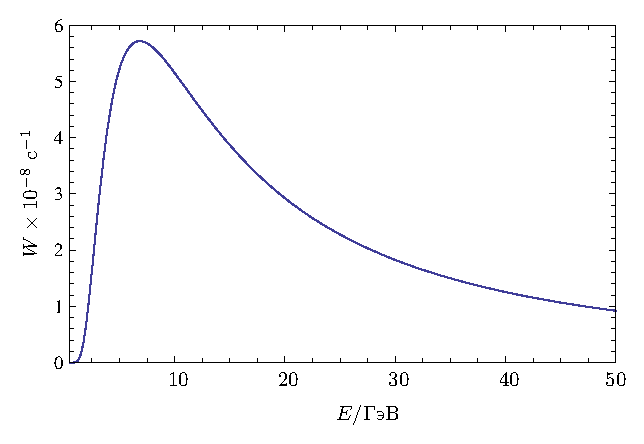
\includegraphics[width=14cm]{fig5_5.eps}}
\caption{Зависимость вероятности рождения электрон-позитронных пар в единицу времени от энергии 
начального электрона  при $B=100B_e$ и $T=1$ кэВ.}
\label{fig:prob}
\end{figure}

Оценивая минимальную длину свободного пробега электрона 
с энергией $E \sim 10^{4} m$ при величинах  
магнитного поля и температуры таких же, как на рис.~\ref{fig:prob}, получим 
$\ell \simeq 57$ см, что 
оказывается много меньше величины зазора $(\sim 100)$ м.  
Вместе с тем изменение числа электронов в потоке за счет рождения пар может быть 
выражено через оптическую толщу $\tau$ следующим образом: 
%
\beq
\label{eq:tau}
N = N_0 \exp{[-\tau]} \simeq N_0 \exp{\left [- \int \limits_0^h d x W \right ]} \, , 
\eeq
\noindent где  $h$ -- ширина электрического зазора, 
$N_0$ -- начальное число электронов в потоке.

Оценивая отношение $N/N_0$ при $h \sim 10^4$ см, $E \sim 10^{7} m$, 
получим $N/N_0 \simeq 0.99$. Таким образом, рассматриваемый 
процесс дает возможность  увеличивать количество $e^+e^-$-плазмы в области 
полярной шапки. Однако детальный количественный анализ 
развития каскада  $e^+e^-$-пар требует 
решения кинетического уравнения, что выходит за рамки нашей задачи.

Наконец, необходимо сделать еще одно замечание.  Резонансы 
на виртуальных электроне и 
фотоне соответствуют тому факту, что указанные частицы становятся 
реальными. Таким образом,  
рассматриваемый процесс схематично можно представить в виде совокупности трех 
подпроцессов: 
\begin{itemize}
\item
поглощение фотона электроном с рождением электрона на первом уровне Ландау, $e_0+\gamma \to e_1$; 

\item
переход электрона с первого уровня на нулевой с испусканием жесткого $\gamma$-кванта, 
$e_1 \to e_0 + \gamma$;

\item
рождение $e^+e^-$-пары жестким фотоном, $\gamma \to e^+e^-$.

\end{itemize}

Парциальные вклады (branching fractions) последних двух 
реакций приближенно равны 1 и $1/2$ соответсвенно 
(множитель $1/2$ возникает от того, 
что в процессе $\gamma \to e^+e^-$ участвует фотон только одной поляризации из двух возможных). 
Поэтому коэффициент поглощения электрона в  процессе  
$\gamma e \to e e^+e^-$ может быть легко получен из 
вероятности перехода $\gamma + e_0  \to e_1$, как $W = W_{\gamma + e_0 \to e_1}/2$. 
При этом вероятность $W_{\gamma + e_0 \to e_1}$ может быть получена из результатов 
работы~\cite{Latal:1986} и согласуется с нашим результатом~(\ref{eq:Wfin}).
 
 